\documentclass[tikz]{standalone}

\usepackage{newtxmath}
\usepackage{tikz}
\usetikzlibrary{decorations.pathmorphing}
\usetikzlibrary{shapes.geometric,positioning}

\begin{document}
	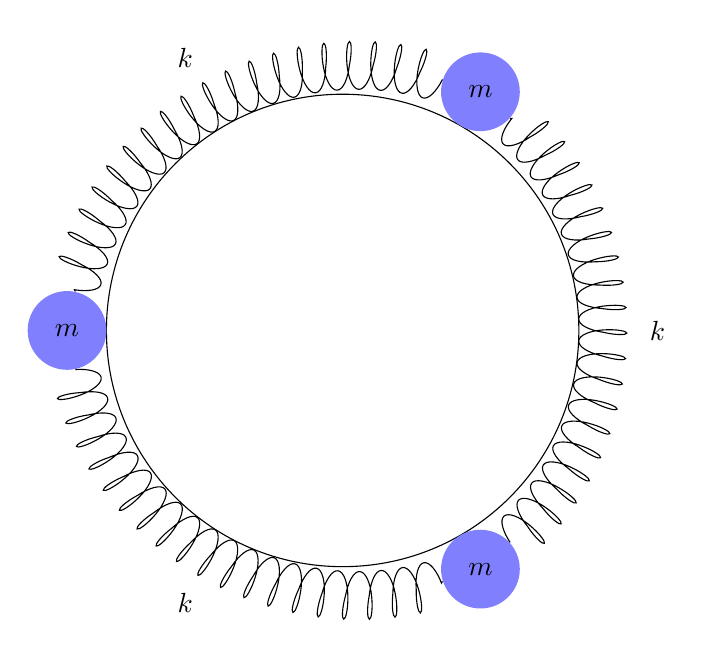
\begin{tikzpicture}
		[defsty/.style={circle ,fill=blue!50, minimum size=1cm},
		arcsty/.style={
			decoration={coil,aspect=0.3,segment length=3mm,amplitude=3mm},
			decorate, draw}]
		\draw (0,0) circle (3cm);
		\node (node 1) at ( 60: 3.5cm) [defsty] {$m$};
		\node (node 2) at (180: 3.5cm) [defsty] {$m$};
		\node (node 3) at (-60: 3.5cm) [defsty] {$m$};
		
		\draw[arcsty] (node 1) to [bend right=48] (node 2);
		\draw[arcsty] (node 2) to [bend right=48] (node 3);
		\draw[arcsty] (node 3) to [bend right=48] (node 1);
		
		\node (text 1) at ( 120: 4cm) [fill=white, line width=0] {$k$};
		\node (text 2) at (-120: 4cm) [fill=white, line width=0] {$k$};
		\node (text 3) at (   0: 4cm) [fill=white, line width=0] {$k$};
	\end{tikzpicture}
\end{document}